%----------------------------------------------------------------------
\documentclass[xcolor=svgnames]{beamer} %, handout
\usetheme{lined}
\usepackage{array}
\usepackage{amsmath}
\usepackage{amssymb}
\usepackage{amsthm}
\usepackage{bbm}
\usepackage[utf8]{inputenc}
\usepackage[T1]{fontenc}
\usepackage{cmbright}   
\usepackage{times}
\usepackage{geometry}
\usepackage[spanish]{babel}
\usepackage{multicol}
\usepackage{tcolorbox}

\usepackage{algorithm2e}

%\usepackage{psfrag}
\usepackage{graphicx}
\usepackage{color}
\usepackage{floatflt}
\usepackage{fancybox}
\usepackage{tabularx}
%\usepackage[all]{xy}
\usepackage{color}
\usepackage{siunitx} % para \degree



\usepackage{tikz}
\usetikzlibrary{positioning}




%\usepackage[most]{tcolorbox}


\theoremstyle{plain}
\newtheorem{definicion}{Definición}



\definecolor{redUnq}{rgb}{.7,.1,.1}
\definecolor{redUnq2}{rgb}{.5,.1,.3}

\mode<presentation>{
	%\usetheme{Boxes}
	%\usecolortheme[RGB={237,132,8}]{structure}
	%\usecolortheme[RGB={205,173,0}]{structure}
	\usecolortheme[RGB={100,10,10}]{structure}

	%\beamertemplateshadingbackground{SteelBlue!70}{Honeydew!10}
	%\usetheme{Warsaw}
	%\usecolortheme{default}
	\usetheme{Singapore}
	%\usetheme{Lined}
	%\usetheme[height=7mm]{Rochester} 
	\setbeamerfont{title}{shape=\bfseries,family=\rmfamily}
	%\usefonttheme[onlylarge]{structuresmallcapsserif}
	%\usefonttheme[onlysmall]{structurebold}
	\setbeamercolor{title}{fg=redUnq,bg=gray!40}
	\usefonttheme{professionalfonts}
	\setbeamercovered{highly dynamic}
	\setbeamercovered{transparent=10}
	\setbeamertemplate{navigation symbols}{}
	\colorlet{structure}{redUnq}

	\setbeamertemplate{frametitle}[default][left]
}

\definecolor{verzul}{rgb}{0, 0.5,0.5}

\renewcommand{\textbf}[1]{{\bfseries\textcolor{redUnq2}{#1}}}
\renewcommand{\emph}[1]{{\em\textcolor{redUnq2}{#1}}}

\setlength{\parindent}{0pt}
\theoremstyle{definition}
\newtheorem{ejem}{Ejemplo}
\newtheorem{defi}{Definición}
\newtheorem{ejer}{Ejercicio}
\newtheorem{prop}{Propiedad}
\newtheorem{lema}{Lema}
\newtheorem{teor}{Teorema}
\newtheorem{coro}{Corolario}

 

\newcommand{\Rset}{\mathbbmss{R}}
\newcommand{\Cset}{\mathbbmss{C}}
\newcommand{\PD}[2]{\frac{\partial #1}{\partial #2}}
\DeclareMathOperator{\tr}{tr}
\DeclareMathOperator{\adj}{adj}
\DeclareMathOperator{\rango}{rango}

\newenvironment{Boxedminipage}%
{\begin{Sbox}\begin{minipage}}%
{\end{minipage}\end{Sbox}\fbox{\TheSbox}}



\title{Métodos Numéricos - Clase 2}
  \logo{
\includegraphics[scale=0.25]{logoUnq} }
\author{Ulises Bussi- Javier Portillo}
%\institute{\scalebox{2}{\includegraphics[scale=0.1]{mdp02.jpg}}} %{Departamento de Ciencia y Tecnología\\ Universidad Nacional de Quilmes\\ }
\date{ $1^\circ$ cuatrimestre 2020} 


%%%%%%%%% Para que al comenzar una section aparezca el Contenido
%\AtBeginSection[]
%{
%  \begin{frame}
%    \frametitle{Contenidos de la Presentación}
%    \tableofcontents[currentsection]
%  \end{frame}
%}




\begin{document} 


\begin{frame} %\thispagestyle{empty}
	\titlepage
\end{frame}

\section{Lo que repito todas las clases}
\begin{frame}
\frametitle{Antes de empezar}
\begin{tcolorbox}
	\begin{defi} \vspace{15pt}

		Un método numérico es un procedimiento que permite obtener, \textbf{de forma aproximada}, solución a un problema, por medio de la aplicación de algoritmos.
	\end{defi}
\end{tcolorbox}


\end{frame}

\section{Introducción}
\begin{frame}
\frametitle{Bracketing Methods.}

Métodos para encontrar raices de funciones de forma numérica.\vspace{10pt}


\begin{tcolorbox}
  \begin{center}
    brackets $\rightarrow$ [ ]
  \end{center}
\end{tcolorbox} \vspace{20pt}
\pause


$"$Encuentra$"$ raices en un intervalo cerrado definido.



\end{frame}

\begin{frame}
\frametitle{Bracketing Methods.}
\textbf{Consideraciones:}
\begin{itemize}
\item Encuentran aproximadamente el valor de la raiz.
\item Requieren definir el intervalo.
\item Requieren que haya solo una raiz en el intervalo.

\end{itemize}
\end{frame}










\section{Método de la Bisección}
\begin{frame}
\frametitle{Método de la bisección}

Basado en el teorema de Bolsano:

\begin{tcolorbox}
\begin{teor}
	Dada $f(x)$ una función continua en el cerrado $[a,b]$ Si $f(a).f(b)<0 \rightarrow c \in [a,b]\, /\, f(c)=0$

\end{teor}
\end{tcolorbox}\vspace{12pt}

\begin{enumerate}
  \item Se propone $\hat c = \frac{a+b}{2} $ como candidato a raiz.
  \item Se evalúa $f(\hat c)$ si $f(\hat c).f(a)>0 \rightarrow  a=\hat c$ (idem b). 
  \item  Se repite hasta llegar a una tolerancia aceptable.
\end{enumerate}

\end{frame}

\begin{frame}
\frametitle{Método de la bisección}

Error relativo en la iteración $i$: $e_i = \frac{|\hat c_i-\hat c_{i-1}|}{\hat c_i} $ $\rightarrow$ $\boxed{ e_i= \frac{b_i-a_i}{b_i+a_i}}$\vspace{10pt}

\textbf{Consideraciones:}
\begin{itemize}
\item El intervalo de busqueda se reduce a la mitad en cada iteración.
\pause
\item El error relativo también!
\pause
\item Podemos calcular el error en cualquier paso $i$ a \textit{priori}.
\pause
\item El error absoluto en un paso $i$ será: $E_i = \frac{b-a}{2^i}$
\end{itemize}

\end{frame}

\subsection{Ejemplo Bisección}
\begin{frame}
\frametitle{Bisección: un ejemplo}
Tomemos $f(x) = -2x^2+8x-5, \, a=2, \, b=5$
\begin{minipage}{.7\linewidth}
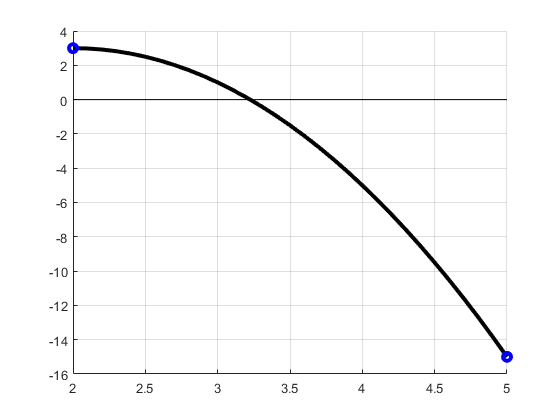
\includegraphics[scale=.5]{Biseccion/f0.png} 
\end{minipage}
\begin{minipage}{.25\linewidth}
$$f(2)=3 \,,\,f(5)=-15$$\vspace{7pt}
$$f(2).f(5) = -45$$\vspace{7pt}

\end{minipage}
\end{frame}

\begin{frame}
\frametitle{Bisección: un ejemplo}
Tomemos $f(x) = -2x^2+8x-5, \, a=2, \, b=5$
\begin{minipage}{.7\linewidth}
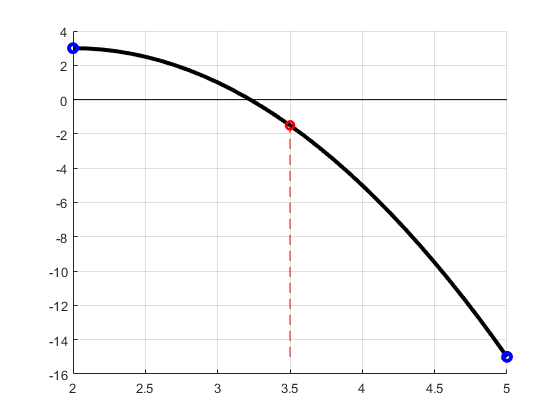
\includegraphics[scale=.5]{Biseccion/f1.png} 
\end{minipage}
\begin{minipage}{.25\linewidth}
$$c_1 = \frac{2+5}{2} = 3.5 $$\vspace{7pt}
$$f(c_1) = -1.5 $$\vspace{7pt}
$$ b = c_1$$
\end{minipage}
\end{frame}

%frame3
\begin{frame}
\frametitle{Bisección: un ejemplo}
Tomemos $f(x) = -2x^2+8x-5, \, a=2, \, b=5$
\begin{minipage}{.7\linewidth}
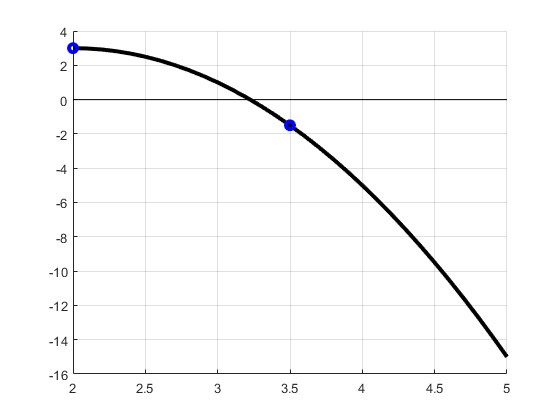
\includegraphics[scale=.5]{Biseccion/f2.png} 
\end{minipage}
\begin{minipage}{.25\linewidth}
$$f(2)=3 \,,\,f(3.5)=-1.5$$\vspace{7pt}
$$f(2).f(1.5) = -4.5$$\vspace{7pt}

\end{minipage}
\end{frame}

\begin{frame}
\frametitle{Bisección: un ejemplo}
Tomemos $f(x) = -2x^2+8x-5, \, a=2, \, b=5$
\begin{minipage}{.7\linewidth}
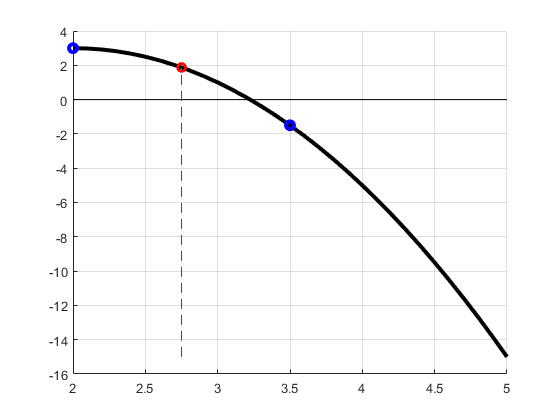
\includegraphics[scale=.5]{Biseccion/f3.png} 
\end{minipage}
\begin{minipage}{.25\linewidth}
$$c_2 = \frac{2+3.5}{2} = 2.75 $$\vspace{7pt}
$$f(c_2) = 1.875 $$\vspace{7pt}
$$ a = c_2$$

\end{minipage}
\end{frame}


%frame5
\begin{frame}
\frametitle{Bisección: un ejemplo}
Tomemos $f(x) = -2x^2+8x-5, \, a=2, \, b=5$
\begin{minipage}{.7\linewidth}
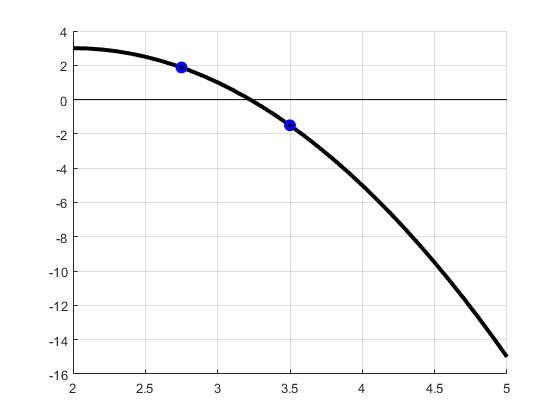
\includegraphics[scale=.5]{Biseccion/f4.png} 
\end{minipage}
\begin{minipage}{.25\linewidth}
$$f(2.75)=1.875 \,,\,f(3.5)=-1.5$$\vspace{7pt}
$$f(2).f(1.5) = -2.81$$\vspace{7pt}
\end{minipage}
\end{frame}


\begin{frame}
\frametitle{Bisección: un ejemplo}
Tomemos $f(x) = -2x^2+8x-5, \, a=2, \, b=5$
\begin{minipage}{.7\linewidth}
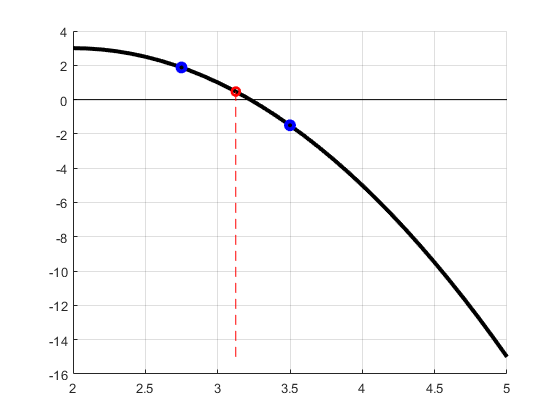
\includegraphics[scale=.5]{Biseccion/f5.png} 
\end{minipage}
\begin{minipage}{.25\linewidth}
$$c_3 = \frac{2.75+3.5}{2} = 3.125 $$\vspace{7pt}
$$f(c_3) = 0.46 $$\vspace{7pt}
$$ a = c_3$$
\end{minipage}
\end{frame}



\section{Método de la Falsa Posición}

\begin{frame}
\frametitle{Método de la Falsa Posición}

Basado en el teorema de Bolsano.\vspace{12pt}


\begin{enumerate}
  \item Se propone $\hat c$ uniendo $f(a)$ y $f(b)$ con una recta y encontrando la raiz de la recta.
  \item Se evalúa $f(\hat c)$ si $f(\hat c).f(a)>0 \rightarrow  a=\hat c$ (idem b). 
  \item  Se repite hasta llegar a una tolerancia aceptable.
\end{enumerate}

\end{frame}

\begin{frame}
\frametitle{Método de la Falsa Posición}

\begin{minipage}{.45\linewidth}
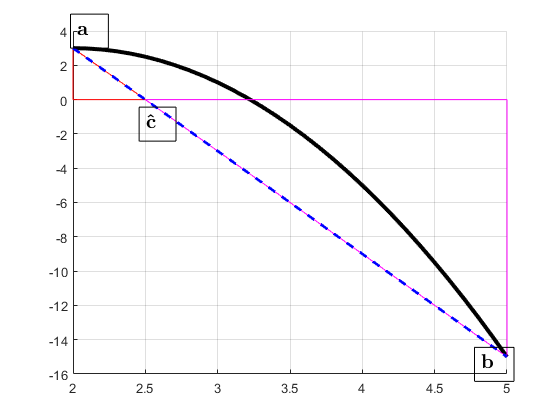
\includegraphics[scale=.35]{FalsaPosicion/triangulosSemejantes.png} 

Se forman dos triangulos semejantes!

\end{minipage} \begin{minipage}{.45\linewidth}

\[\arraycolsep=1pt\def\arraystretch{2}
\begin{array}{ccc}
\frac{f(a)}{c-a} & = & \frac{f(b)}{c-b} \\
f(a)(c-b) & = & f(b)(c-a)\\
c [f(a)-f(b)] & = & f(a)b - f(b)a \\\vspace{5pt}
c & = & \frac{f(a)b-f(b)a}{f(a)-f(b)}\\
c & = & \frac{ f(a)b-f(b)a {\color{red} +f(a)a-f(a)a }  }{ f(a)-f(b) }\\
\end{array}
\]
$$ \boxed{ c  = a + f(a)\frac{b-a}{f(a)-f(b)} } $$


\end{minipage}
\end{frame}





\subsection{Ejemplo Falsa Posición}

\begin{frame}
\vspace{-5pt}
\frametitle{Falsa Posición: un ejemplo}
Tomemos $f(x) = -2x^2+8x-5, \, a=2, \, b=5$
\begin{minipage}{.7\linewidth}
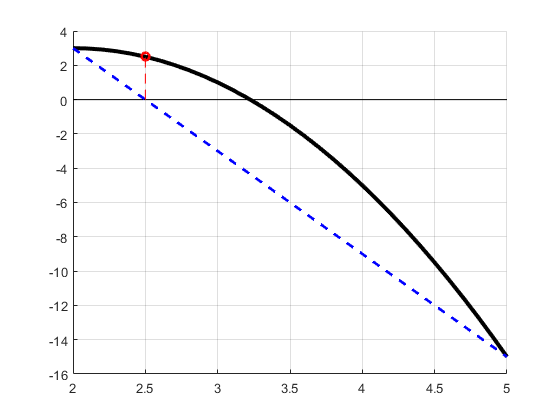
\includegraphics[scale=.45]{FalsaPosicion/f1.png} 
\end{minipage}
\begin{minipage}{.25\linewidth}
$$f(2)=3 \,,\,f(5)=-15$$
$$f(2).f(5) = -45$$
$$c_1 = 2 +3\frac{5-2}{3-(-15)}$$
$$c_1 = 2.5 $$
$$f(c_1) = 2.5 $$
$$ a = c_1$$\vspace{-5pt}
\end{minipage}\vspace{-5pt}
\textbf{Todos los numeros truncados a dos decimales para que se vean las cuentas!}
\end{frame}

%frame2
\begin{frame}
\frametitle{Falsa Posición: un ejemplo}
Tomemos $f(x) = -2x^2+8x-5, \, a=2, \, b=5$
\begin{minipage}{.65\linewidth}
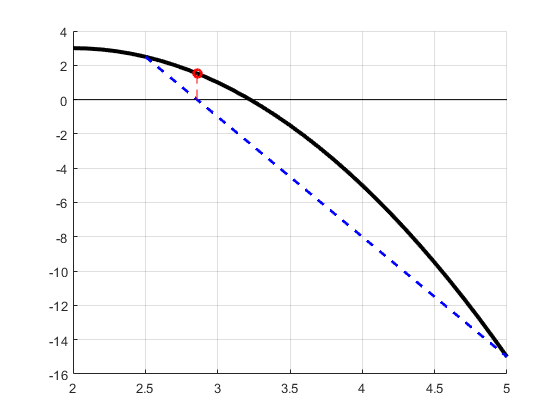
\includegraphics[scale=.45]{FalsaPosicion/f2.png} 
\end{minipage}
\begin{minipage}{.25\linewidth}
$$f(2.5)=2.5 \,,\,f(5)=-15$$\vspace{7pt}
$$c_2 = 2.5 +2.5\frac{5-2.5}{2.5-(-15)}$$
$$c_2 = 2.86 $$
$$f(c_2) = 1.53 $$
$$ a = c_2$$\vspace{-5pt}

\end{minipage}\vspace{-5pt}
\textbf{Todos los numeros truncados a dos decimales para que se vean las cuentas!}

\end{frame}


%frame3
\begin{frame}
\frametitle{Falsa Posición: un ejemplo}
Tomemos $f(x) = -2x^2+8x-5, \, a=2, \, b=5$
\begin{minipage}{.65\linewidth}
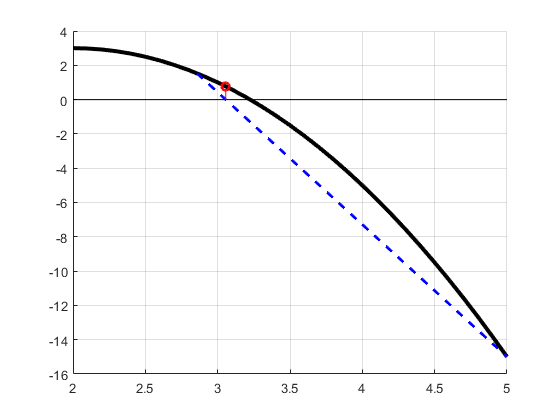
\includegraphics[scale=.45]{FalsaPosicion/f3.png} 
\end{minipage} \hspace{-15pt}
\begin{minipage}{.25\linewidth}

$$\begin{array}{ccc}
f(2.85)&=&1.53 \\
f(5)&=&-15 \\

c_3 &=& 2.85 + \\
    & &+ 1.53\frac{5-2.85}{1.53-(-15)} 
\end{array} $$
$$c_3 = 3.05 $$
$$f(c_3) = 0.77 $$
$$ a = c_3$$\vspace{-5pt}

\end{minipage}

\vspace{-3pt}
\textbf{Todos los numeros truncados a dos decimales para que se vean las cuentas!}

\end{frame}

\subsection{Consideraciones}

\begin{frame}
\frametitle{Falsa Posición}

Error relativo en la iteración $i$: $e_i = \frac{|\hat c_i-\hat c_{i-1}|}{\hat c_i} $



\textbf{Consideraciones:}
\begin{itemize}
  \item El intervalo de busqueda \textbf{NO} se reduce a la mitad en cada iteración.
  \pause
  \item La convergencia de este método suele ser más rápida aunque el intervalo de   busqueda no reduce acorde con esto.
  \pause
  \item Con determinadas funciones la convergencia es lenta.
\end{itemize}

\end{frame}


\begin{frame}
\frametitle{Falsa Posición}

$$f(x) = e^{ (x-2)^2} - 15 $$
\begin{minipage}{.55\linewidth}
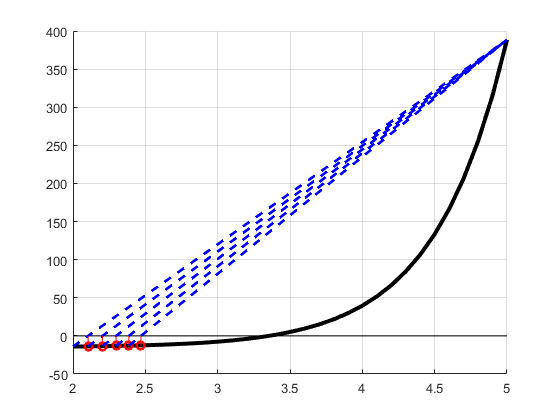
\includegraphics[scale=.45]{FalsaPosicion/malaConvergencia.png}
\end{minipage}
\begin{minipage}{.4\linewidth}
Este es un ejemplo de donde pude ocurrir la mala convergencia.


\end{minipage}

\end{frame}



\section{Criterios de parada}

\begin{frame}
\frametitle{Criterios de parada}
¿Cuándo nos detenemos?
\pause
\begin{itemize}
\item El error absoluto llega a un valor aceptable (el intervalo en el cual busco la raiz se achicó x. ej. a $1e-4$).
\pause
\item El error relativo del paso deja de ser significante (x. ej. el error relativo disminuye menos de $0.1\%$ en cada iteración).
\pause
\item El numero de iteraciones supera un número máximo  (x. ej. $1000$ iteraciones).
\end{itemize}

\end{frame}




\end{document}

%%% Local Variables: 
%%% mode: latex
%%% TeX-master: t
%%% End: 







